\section{Error State Extended Kalman Filter}
\label{error_state_extended_kalman_filter}

The previous section introduced the Extended
Kalman Filter, which uses local linearization as a way to allow us to apply the Kalman
filter equations to non-linear systems. In this section, we are going to look
at a variant of the EKF called the Error-State Extended
Kalman Filter, or ES-EKF, which has a couple of nice properties. 

By the end of this section, you should be able to describe the error state
formulation of the Extended Kalman Filter, and describe the advantages of the error state EKF
over the vanilla EKF that you learned about in the
previous video. 

The idea behind
the error state EKF is really very simple. We are going to start thinking about our vehicle state, $\mathbf{x}$, as being composed
of two parts; 

\begin{itemize}
\item A large part called the nominal state, $\hat{\mathbf{x}}$
\item A small part called the error state $\delta \mathbf{x}$
\end{itemize}

We can think of a simple example of tracking the position of a car over time. The green line in Figure \ref{es_extended_kalman_filter_1} shows the true position
of the car, which is the quantity we're trying to estimate. 

\begin{figure}[!htb]
\begin{center}
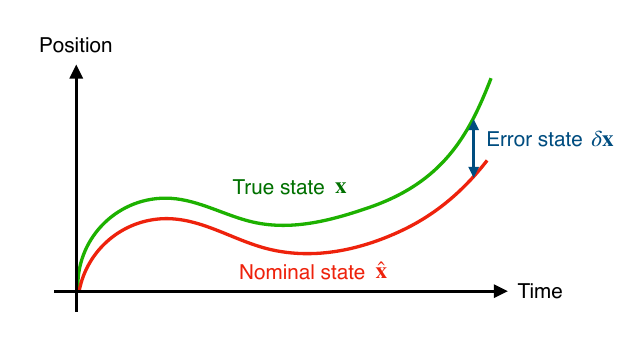
\includegraphics[scale=0.280]{img/kalman_filter/es_extended_kalman_filter_1.jpeg}
\end{center}
\caption{State error $\delta \mathbf{x}$.}
\label{es_extended_kalman_filter_1}
\end{figure}

The red line is the nominal state, or our best guess what the true state could
be based on what we know about the car's motion model and acceleration and breaking inputs. 

Of course, our motion model is never perfect, and there is always some random process noise. These errors build up over time as we integrate
the motion model. We can think of the error state as the place where all of these modelling errors and process noise
accumulate over time, so that the error state is just the difference between the nominal state and the true state at any given time. 
If we can figure out what the error state is, we can actually use it as a correction to the nominal state to bring us closer to
the true state. 

So, in the error state EKF, instead of doing Kalman filtering on the full state
which might have lots of complicated non-linear behaviors, we are going to use the EKF to estimate the error
state instead, and then use the estimate of the error state as a correction to the nominal state. 

What this means mathematically is that we are going to rearrange our
linearized motion model so that we now have an equation that can tell us how the difference between the true state at time, $k$, and our predicted
state at time, $k$, is related to the same difference at time, $k-1$. These differences
are exactly the error states we just talked about; $\delta \mathbf{x}_k$  and
$\delta \mathbf{x}_{k-1}$, 

\begin{equation}
\mathbf{x}_k = \mathbf{f}(\hat{\mathbf{x}}_{k-1}, \mathbf{u}_{k-1}, \mathbf{0}) + \mathbf{F}_{k-1}(\mathbf{x}_{k-1} - \hat{\mathbf{x}}_{k-1}) + \mathbf{L}_{k-1}\mathbf{w}_{k-1}
\end{equation}

\begin{eqnarray}
\delta \mathbf{x}_{k-1} = \mathbf{x}_{k-1} - \hat{\mathbf{x}}_{k-1} \\
\delta \mathbf{x}_{k} = \mathbf{x}_{k} - \mathbf{f}(\hat{\mathbf{x}}_{k-1}, \mathbf{u}_{k-1}, \mathbf{0})
\end{eqnarray}

\begin{framed}
\theoremstyle{remark}
\begin{remark}{\textbf{Error State Kinematics}}

The equations relating $\delta \mathbf{x}_k$  and $\delta \mathbf{x}_{k-1}$  are called the error state kinematics.
\end{remark}
\end{framed}

We can also re-express our linearized measurement model in terms of the error state directly. 
We can use this error state formulation of the EKF in a very similar way to the vanilla EKF. 

We start off by updating the nominal state using the non-linear motion model and our current best
estimate of the state. We could do this a bunch of times before ever getting a measurement for the correction step. So, the current
best estimate might be $\check{\mathbf{x}}$ or $\hat{\mathbf{x}}$. 

\begin{eqnarray}
\check{\mathbf{x}}_{k} = \mathbf{f}(\hat{\mathbf{x}}_{k-1}, \mathbf{u}_{k-1}, \mathbf{0})
\end{eqnarray}

We also need to keep track of the state covariance, which grows as
we integrate more and more process noise from the motion model. Note that again, the previous
covariance estimate could be $\check{\mathbf{P}}$  or $\hat{\mathbf{P}}$ depending
on whether we used a measurement to do a correction step. 

\begin{eqnarray}
\check{\mathbf{P}}_{k} = \mathbf{F}_{k-1}\mathbf{P}_{k-1}\mathbf{F}_{k-1}^T + \mathbf{L}_{k-1}\mathbf{Q}_{k-1}\mathbf{L}_{k-1}^T
\end{eqnarray}

We can repeat the loop updating the nominal state and the error state covariance for as long as we like until we receive
the measurement and want to do a correction. When this happens, we can compute the Kalman gain 

\begin{eqnarray}
\mathbf{K}_{k} = \check{\mathbf{P}}_{k-1}\mathbf{H}_{k}^T(\mathbf{H}_{k}\check{\mathbf{P}}_{k}\mathbf{H}_{k}^T + \mathbf{R})^{-1}
\end{eqnarray}

Then compute the best estimate of the error state using
the Kalman gain, the measurement, and our nonlinear measurement model. 

\begin{eqnarray}
\delta \hat{\mathbf{x}}_{k} = \mathbf{K}_{k}(\mathbf{y}_{k} - \mathbf{h}_{k}(\check{\mathbf{x}}_{k},\mathbf{0}) )
\end{eqnarray}

Once we have an estimate for the mean of the error state, we want to use this to update the nominal state and
correct the error. We can do that by just adding our estimate of the error state to the nominal state to get the correct state estimate for the full state. 

\begin{eqnarray}
\hat{\mathbf{x}}_{k} = \check{\mathbf{x}}_{k} + \delta \hat{\mathbf{x}}_{k}
\end{eqnarray}

Finally, we can update the state covariance using the usual equations.

\begin{eqnarray}
\hat{\mathbf{P}}_{k} = (\mathbf{I} - \mathbf{K}_{k} \mathbf{H}_{k})\check{\mathbf{P}}_{k}
\end{eqnarray}

\textbf{Advantages of ES-EKF}

This process goes on forever. So, why would we actually want to use the error state EKF
in practice? Well, there are two good reasons to use it. 

\begin{itemize}
\item One reason is that it can often work better than the vanilla EKF because the small error
state is more amenable to linear filtering than the large nominal state, which we can integrate non-linearly. 
\item The other reason is that the error state formulation makes it much easier to work with constrained quantities like rotations. 
The reason for this is that we do not necessarily have to use plane vector addition to break down the state. In fact, we could use any generalized
composition operation we like as long as it gives us a consistent way of incorporating small perturbations into the nominal state. 
\end{itemize}

In summary, the error state formulation of the EKF separates the vehicle state into a large nominal state and a small error state. The nominal state
keeps track of what the motion model predicts the states should be, while the error state captures the
modelling errors and process noise that accumulate over time. In the error state EKF, we estimate
this small error state and use it as a correction to the nominal state. This is the main
difference between the error state EKF and the vanilla EKF, which estimates the full state. Keep in mind that both formulations still rely on
local linearization. The error state EKF has a couple of advantages over the vanilla EKF. The first is that it simply performs better because
the evolution of the error state tends to be closer to linear. The other is that the error state formulation makes it easier to handle special quantities like 3D rotations. 
\section{Questions}
\section{Assignements}
